
% GENERAL
\documentclass{beamer}
%\usepackage[catalan]{babel}
\usepackage[latin1]{inputenc}
%\usepackage[utf8]{inputenc} % Required for inputting international characters
\usepackage[T1]{fontenc} % Output font encoding for international characters

\usepackage{mathpazo} % Use the Palatino font by default
\usepackage{xcolor}

\usepackage{hyperref}
\usepackage{url}
\usepackage{dirtree}
\usepackage[font=small]{caption}
\captionsetup{justification=raggedright,singlelinecheck=false}
\usepackage{subcaption}
\usepackage{rotating}
\usepackage{float}
\usepackage{multicol}

\usepackage[backend=bibtex,
					 style=numeric,
					 natbib=true,
					 sorting=none]{biblatex} % Use the bibtex backend with the authoryear citation style (which resembles APA)

\addbibresource{bibliography.bib} % The filename of the bibliography

\usepackage[autostyle=true]{csquotes} % Required to generate language-dependent quotes in the bibliography

%----------------------------------------------------------------------------------------------------------------
%  BEAMER
%----------------------------------------------------------------------------------------------------------------

\usetheme{Madrid}
\usecolortheme{beaver} 
\setbeamercolor{item projected}{bg=darkred}

 \AtBeginSection[]
{
  \begin{frame}
    \frametitle{}
    \tableofcontents[currentsection,hideallsubsections]
  \end{frame}
}

%----------------------------------------------------------------------------------------
%	TITLE PAGE
%----------------------------------------------------------------------------------------
  
\title[Man-made Structures Detection]{Man-made Structures Detection from Space}
\subtitle[Fundamentals of Data Science Master's Thesis]{Fundamentals of Data Science Master's Thesis}
\author[E. Ribas, P. Weber]{Eduard Ribas, Peter Weber \\ \hspace{1cm}  \\  \textit{Advisor}: Dr. Jordi Vitri�  \inst{1}}
\institute[UB]{
  %\inst{1}
  %Facultat de Matem�tiques i Inform�tica, \\
  %Universitat de Barcelona
  %\and
  \inst{1}
  Departament de Matem�tiques i Inform�tica, \\
  Universitat de Barcelona
}
\date[\today]{Barcelona, \today}
\logo{
\includegraphics[width=1cm]{data/ub.png}}
 
%----------------------------------------------------------------------------------------------------------------

\begin{document}
 
\frame{\titlepage}
 
 %----------------------------------------------------------------------------------------------------------------
 
\begin{frame}
\frametitle{Initial frame}
Just some initial content...
\end{frame} 

%----------------------------------------------------------------------------------------------------------------
  
\begin{frame}
\frametitle{Outline}
\begin{multicols}{2}
\tableofcontents%[hideallsubsections]
\end{multicols}

\end{frame} 

%----------------------------------------------------------------------------------------------------------------
 
\section{Introduction}

\subsection{Motivation}
\begin{frame}[allowframebreaks]
\frametitle{Motivation}

Human kind exerts an ever increasing pressure on natural and ecological systems due to the associated consequences of the explosion of human population. The exploitation of the earth manifests itself in extraction of natural res ources, proliferation of human-made infrastructure and waste, and increasing production land use for crop and pastry land \parencite{kareiva2007}. As a logical consequence, we observe widespread declines in biodiversity \parencite{newbold2015}, decrease in natural habitat, attrition of wilderness areas, deforestation, and enhanced emission of greenhouse gases to the atmosphere. This increasing intrusion leads to reduction of benefits that humans receive from natural systems \parencite{costanza2014} such as the extinction of natural resources, and ultimately provoke natural disaster induced by effects such as climate change. 

\end{frame}

\subsection{Satellogic}
\begin{frame}[allowframebreaks]
\frametitle{Satellogic}

This work has been developed in cooperation with Satellogic, a company that provides earth observation data and analytics as a service to enable better decision making for industries, governments, and individuals. Satellogic was founded in 2010 in Buenos Aires, and has expanded since then with offices in Barcelona and China. Satellogic builds, launches and maintains their own satellites.

\end{frame}

\subsection{Thesis goal and outline}
\begin{frame}[allowframebreaks]
\frametitle{Thesis goal and outline}

The motivation for this Master's thesis is to provide an answer to the question:
\begin{itemize}
	\item[] \textit{What is the optimal resolution to detect human impact in satellite imagery, having in mind the economical cost of acquiring and processing the information?} 
\end{itemize}

\end{frame}

%----------------------------------------------------------------------------------------------------------------
 
\section{Datasets}

\subsection{USGS datasource}
\begin{frame}[allowframebreaks]
\frametitle{USGS datasource}

\begin{figure}[h!]
	\centering
	\captionsetup{width=1\linewidth}
	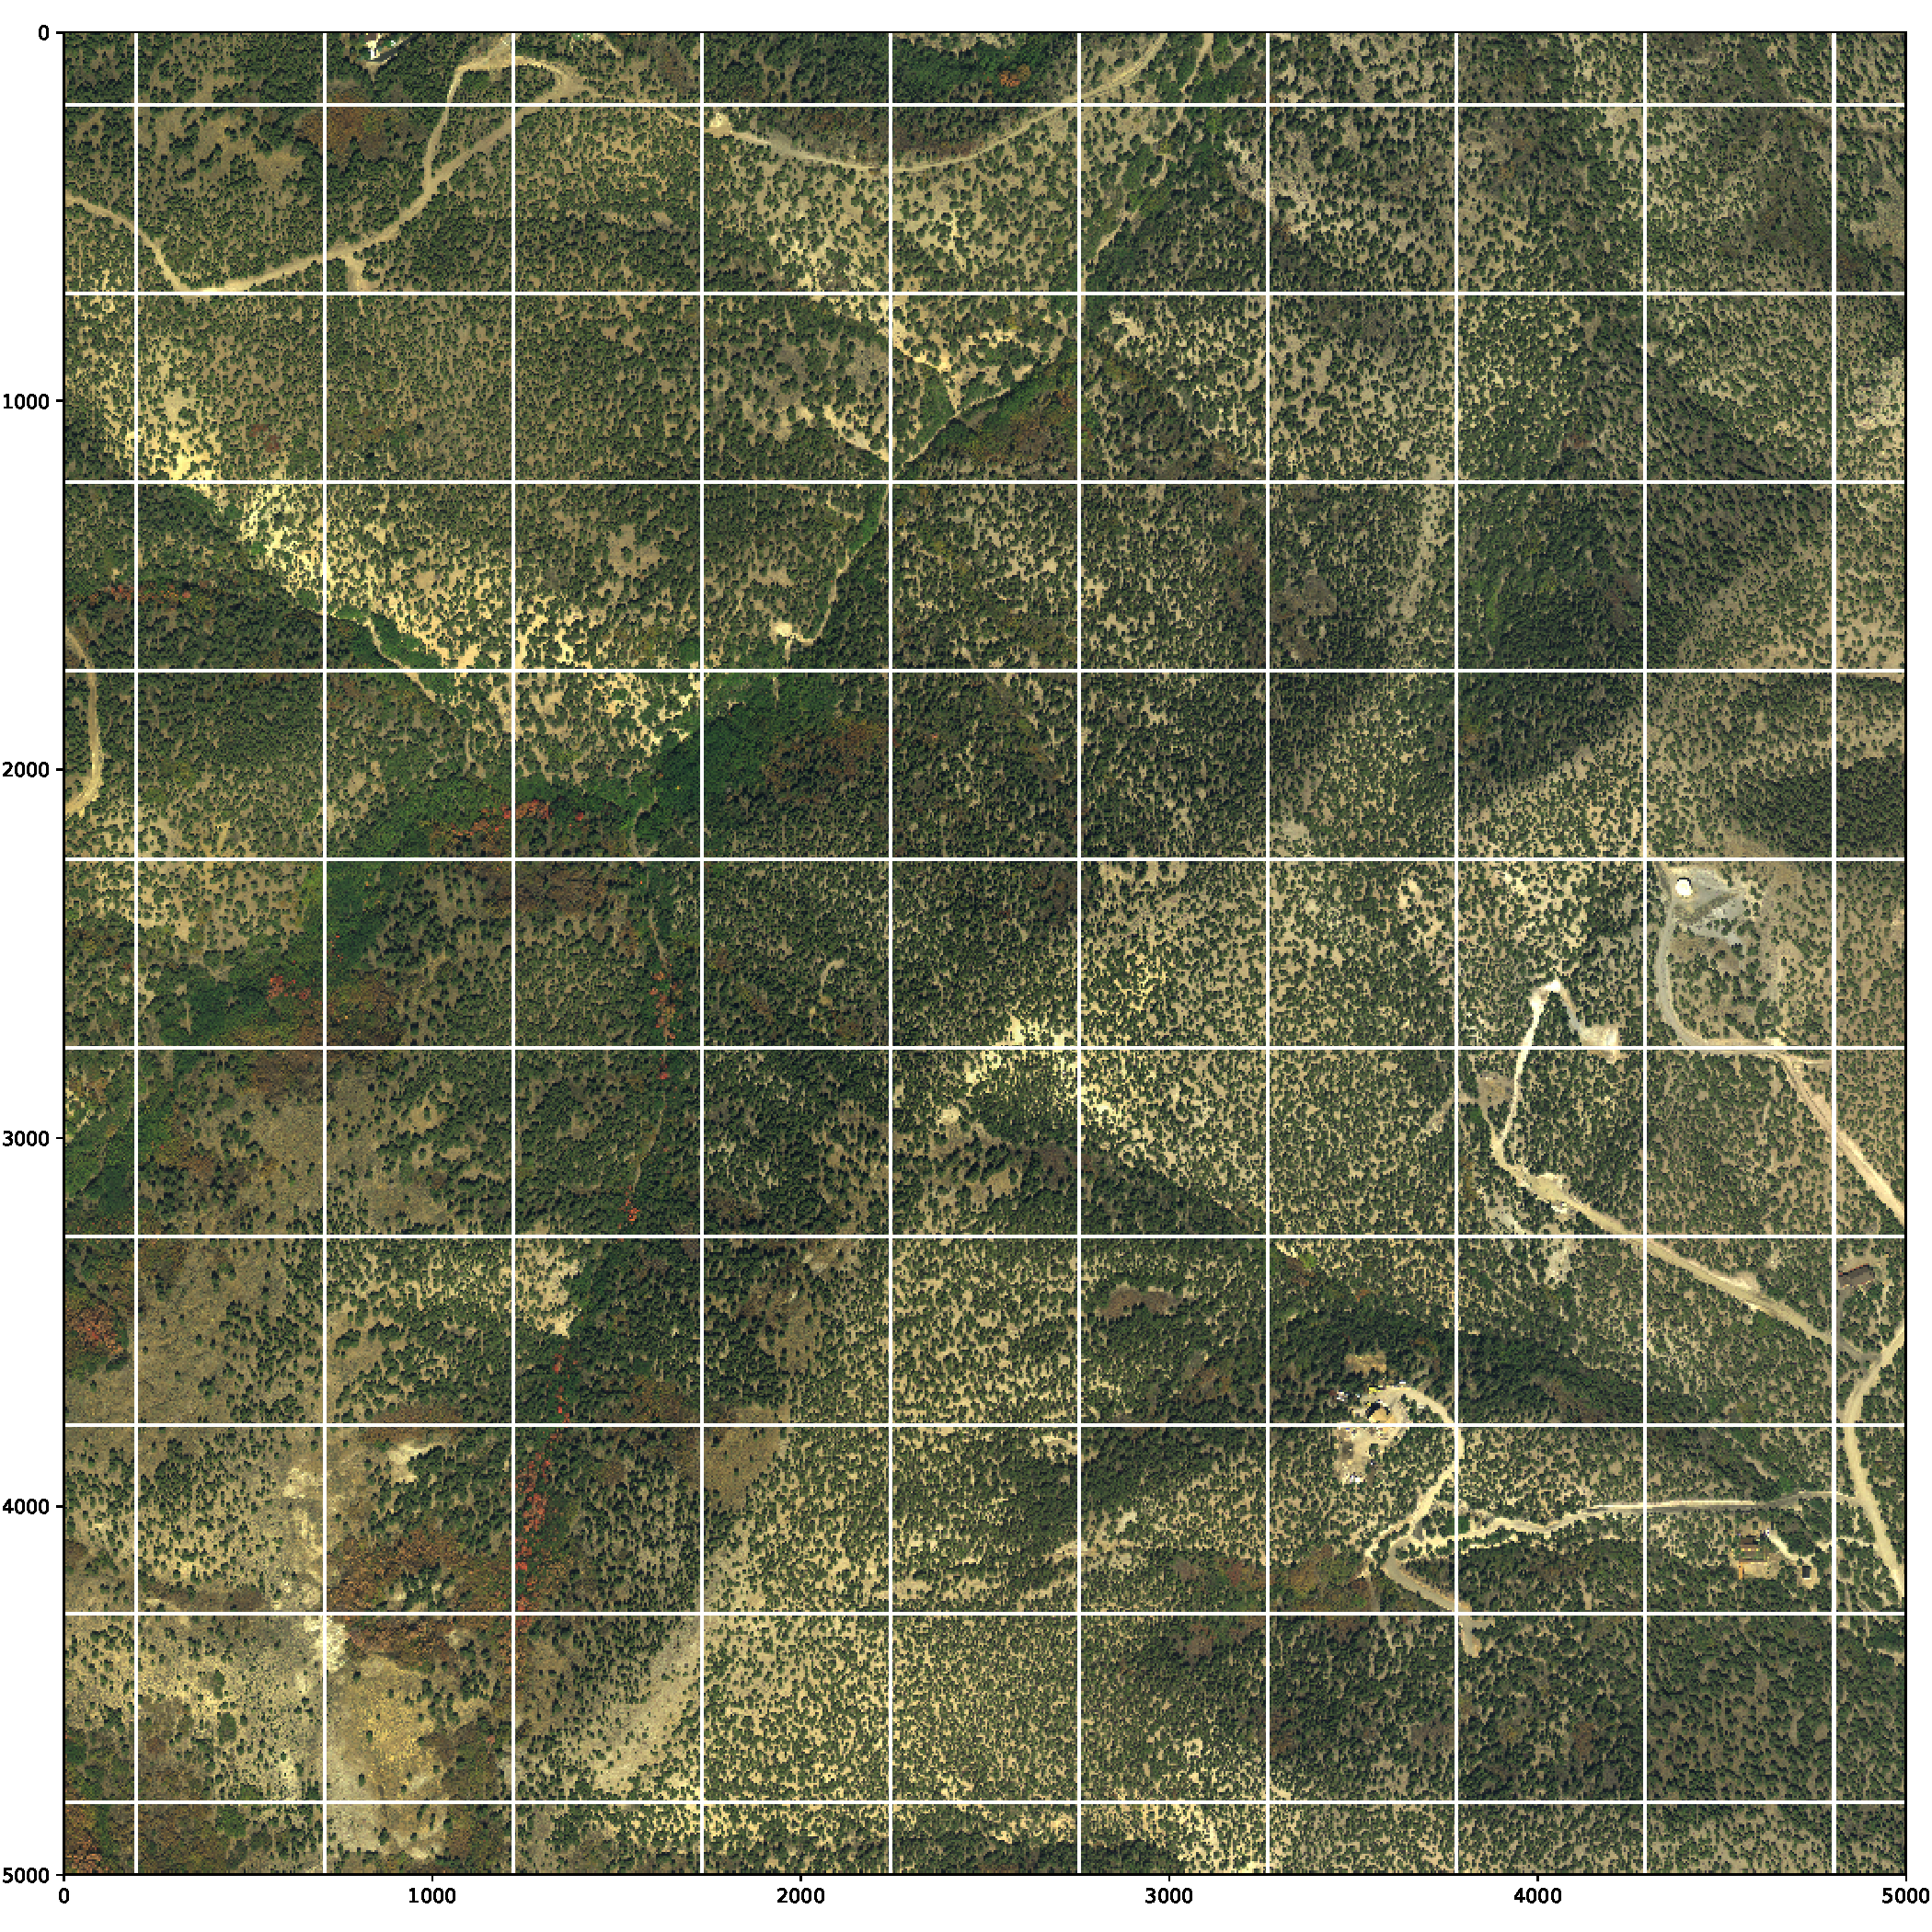
\includegraphics[width=0.4\textwidth]{../report/Figures/example_unproc.pdf}
	\caption{\textbf{Example of unprocessed image.} This image has a size of $5000\times5000$ pixels. The continuous white lines show how we crop smaller images of size $512\times512$ pixels from the original one.}
	\label{fig:example-unproc}
\end{figure}

\end{frame} 

%----------------------------------------------------------------------------------------------------------------

\section{Deep Learning}

\subsection{ResNet}
\begin{frame}
\frametitle{ResNet}

\begin{columns}
 
\column{0.4\textwidth}

\begin{figure}[h!]
	\centering
	\captionsetup{width=1\linewidth}
	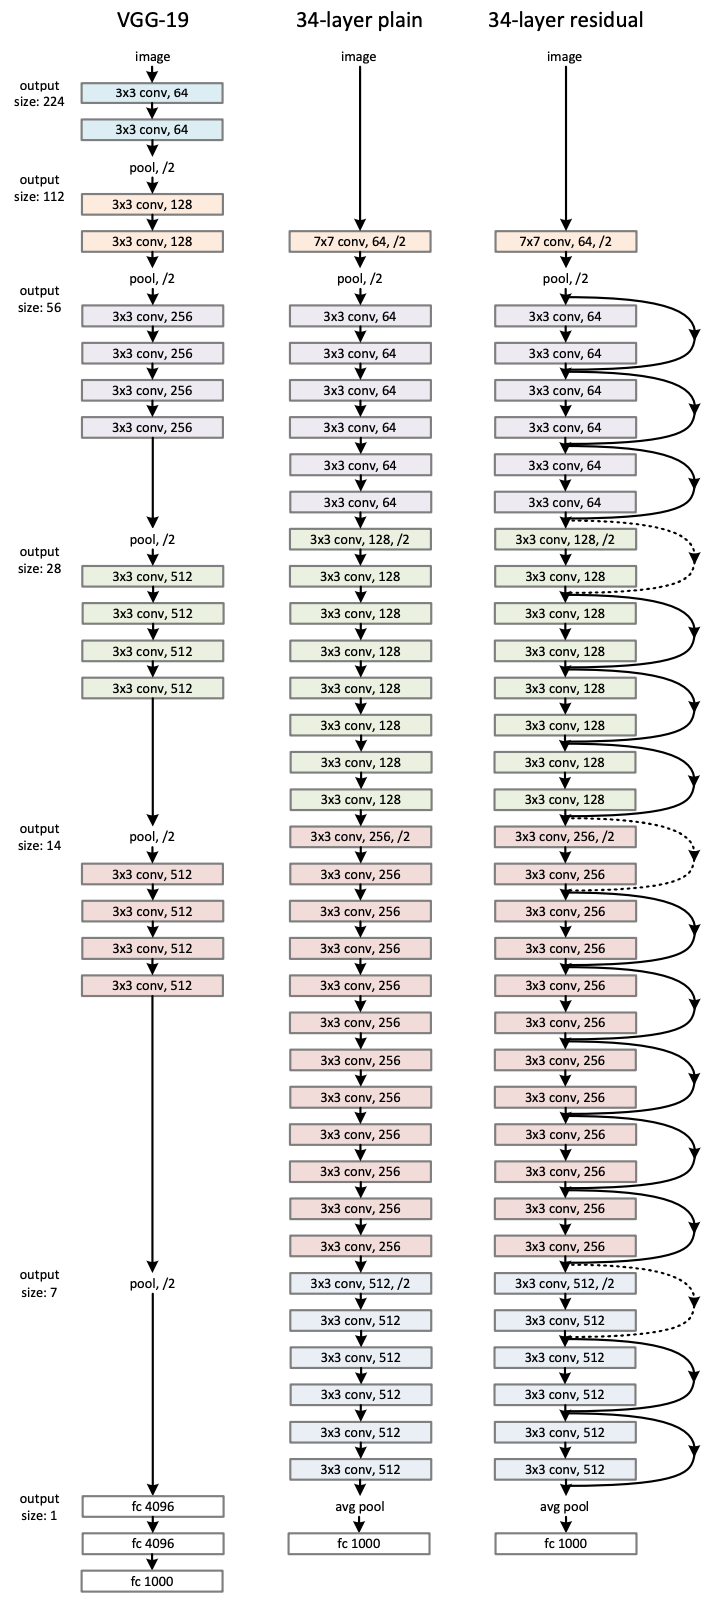
\includegraphics[width=0.6\textwidth]{../report/Figures/resnet_architecture.png}
	\caption{\textbf{Comparison between deep Convolutional Neural Network architectures.} On the left we have a VGG network with 19 layers, in the center a plain CNN with 34 layers, and on the right a ResNet with 34 layers containing residual connections. Figure is adapted from\parencite{he2015}.}
	\label{fig:resnet}
\end{figure}

\column{0.6\textwidth} 

ResNet architecture

\end{columns}

\end{frame} 

%----------------------------------------------------------------------------------------------------------------

\section{Proposed approach}

\subsection{ResNet activations}
\begin{frame}[allowframebreaks]
\frametitle{ResNet activations}

\begin{figure}[H]
	\centering
	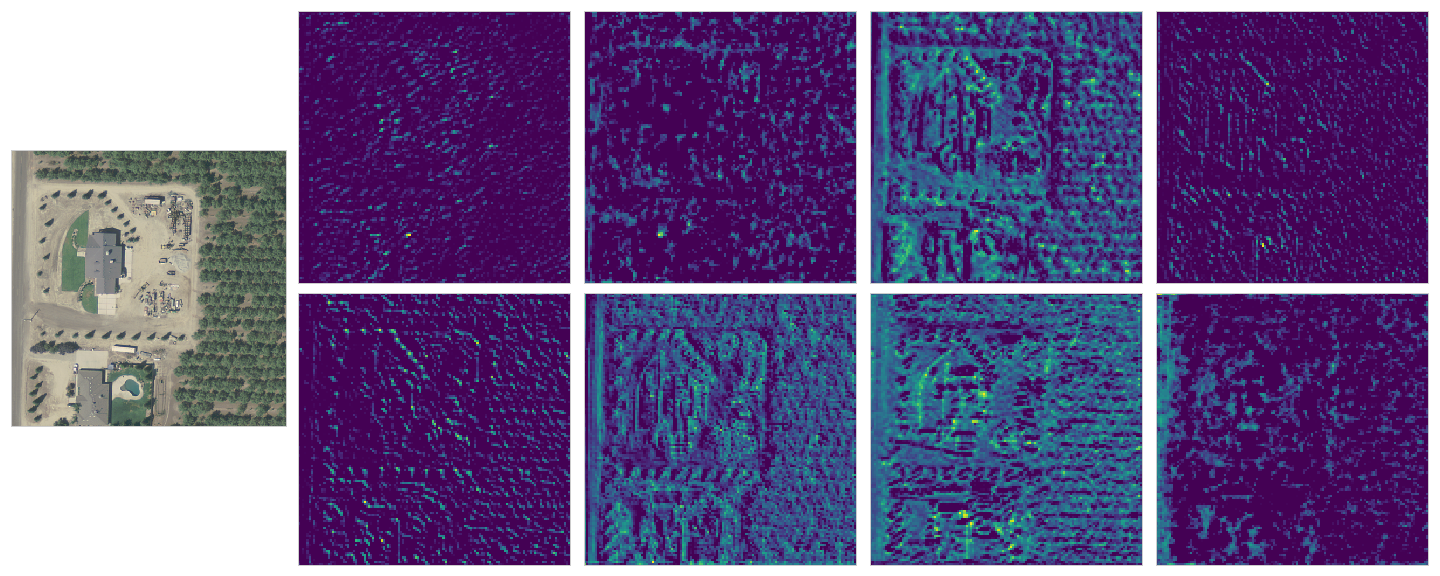
\includegraphics[width=0.9\textwidth]{../report/Figures/activations/agriculture_l2_s1_activation_10.png}
	\captionsetup{width=1\linewidth}
	\caption{\textbf{ResNet activations of an Agriculture image: $10^{th}$ layer.}}
	\label{fig:act_agriculture}
\end{figure}

\begin{figure}[H]
	\centering
	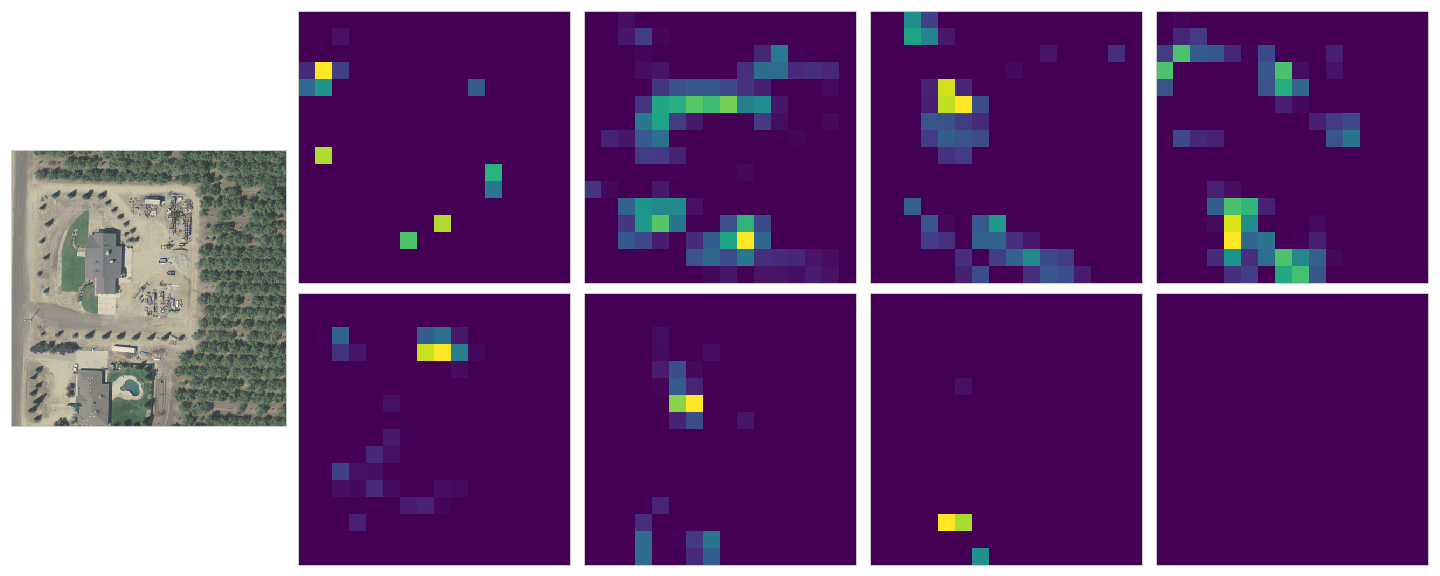
\includegraphics[width=0.9\textwidth]{../report/Figures/activations/agriculture_l2_s1_activation_49.png}
	\captionsetup{width=1\linewidth}
	\caption{\textbf{ResNet activations of an Agriculture image: final layer, $49^{th}$.}}
	\label{fig:act_agriculture}
\end{figure}

\begin{figure}[h!]
	\centering
	\includegraphics[width=\textwidth]{../report/Figures/results/convergence_plots_03m.png}
	\captionsetup{width=1\linewidth}
	\caption{\textbf{Convergence plots of some experiments on the $0.3m$ dataset, for base ($0.3m$) and lowest ($4.8m$) resolutions, and considering $100$ and $200$ neurons.} The models converge more smoothly for lower resolutions, were there are fewer parameters to be fitted.}
	\label{fig:conv_plots_03m}
\end{figure}

\end{frame} 

%----------------------------------------------------------------------------------------------------------------

\section{Results}

\subsection{Man-made structures detection at different scales}
\begin{frame}[allowframebreaks]
\frametitle{Man-made structures detection at different scales}

\begin{figure}[h!]
	\centering
	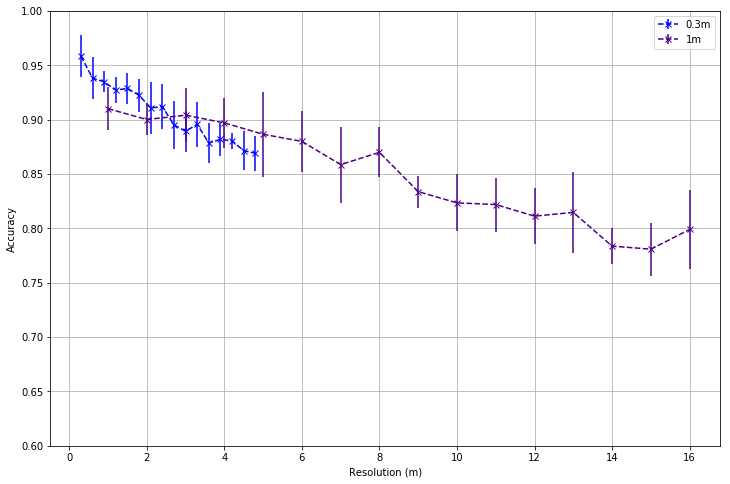
\includegraphics[width=0.8\textwidth]{../report/Figures/results/acc_res_03m_1m.png}
	\captionsetup{width=1\linewidth}
	\caption{\textbf{Accuracy at each resolution for all datasets and architectures.} Similar results are obtained at the same degraded resolutions. The vertical lines represent the variability (standard deviation) for the different the cross-validations folds.}
	\label{fig:acc_res_03m_1m}
\end{figure}

\end{frame} 

%----------------------------------------------------------------------------------------------------------------

\section{Conclusions}

\subsection{The Problem}
\begin{frame}[allowframebreaks]
\frametitle{The Problem}

The intial phase during the development of the project consisted on clearly defining the problem to study. The goal was to investigate which satellite imagery resolutions allowed for an accurate detection of man-made structures, and what would be the cost associated. For that, we needed to define the scope of human activity to consider, look for suitable datasets for this study (which eventually lead to building our own datasets), and define the actual technical problem to be modeled, in order to evaluate the accuracy by resolution. 

Both for the datasets and the problem, we needed them to be feasible enough to not require high technical and computational efforts (which would be, for instance, trying to detect every type of human activity in the images, providing their position and shape, and classifying them into several more categories). On the other hand, we needed it to be a realistic situation, so the results obtained could be extrapolated to other, more complex scenarios.

All in all, having a well-defined problem scope and a good approach to tackle it allowed us to achieve remarkable and realistic results.

\end{frame} 

\subsection{The Datasets}
\begin{frame}[allowframebreaks]
\frametitle{The Datasets}

After investigating existing datasets of labeled satellite images, we could not find the one suitable for our purpose, as most of them were mainly focused towards urban areas, or were just build for some other different goal that would not work for us. Hence, we decided to build it ourselves. It had to be representative enough to pose a challenge for our models, yet feasible to be build with our available time and resources. The four categories considered (agriculture, shrubland-grassland, semi-desert, and forest-woodland) and the balance between non-existent and existent human impact images allowed us to build a good and representative dataset, which makes reasonable to eventually generalize the results obtained to other scenarios.

Of course, we acknowledge that having a larger dataset of images, annotated with higher degree of detail, like position, shapes and types of man-made or natural structures, would be great to build high performance models, capable of detecting all sorts of human impact with far better accuracy. Nevertheless, this high-precision goal could not be fitted into our general purpose.

\end{frame} 

\subsection{The Models and Results}
\begin{frame}[allowframebreaks]
\frametitle{The Models and Results}

Using a pre-trained CNN like the ResNet helped us to speed up the training process and achieve good results without requiring a very large dataset and computational power. The binary classification problem considered turned out to be feasible and representative of how accuracy is affected with a decrease in the image resolution. 

From the results we observe that, as expected, the higher the resolution the better, but also that there seems to be sweet spot between $1$-$2m$ and $8m$ where, except for the more subtle forms of human activity, most of the man-made structures studied are detectable with good accuracy. This trade-off with the resolution allows to consider more cost-economic satellite solutions without dramatically compromising accuracy and utility. For instance, operating a satellite at $2m$ (or $8m$) instead of $1m$ reduces the cost approximately by a factor 6 (or $100$).

\end{frame} 

\subsection{Future work}
\begin{frame}[allowframebreaks]
\frametitle{Future work}

With all that said, we realize that there is still plenty of space for further work and investigations, so let us now indicate some of these ideas.

\begin{itemize}
	\setlength\itemsep{1.5em}

	\item First of all, having a better dataset could help improving the results and open new investigation lines to explore. It could be improved and enlarged with more variate images, with a better and more consistent classification, and including more detailed annotations of the position and type of objects or structures appearing. This would allow to train more accurate models capable of detecting all these kind of human impact.
	
	\item Regarding the model, other techniques for feature extraction could be studied, like other pre-trained Neural Networks, and the parameters itself (like the number of activations to consider, the architecture of the model or the training phase) could be further fine-tuned. Additionally, the pipeline could be made more robust so that it could ingest a larger amount of data, as part of the improvements suggested for the dataset. And, of course, having a powerful computational cluster would allow to speed up the processes and target more ambitious goals.

	\item A more in depth study of the results could help to understand more precisely on which images the algorithms fail, what kind of information are learning (patterns, colors, shapes, etc) and how to enhance them.

	\item Finally, it would be interesting to have a more detailed analysis of the costs associated to all this solution, from data gathering, processing and modeling to the production implementation itself. Also, taking into account other related factors, like infrastructure needed, legal aspects and ecological footprint \parencite{Strubell2019} would give a more complete idea of the viability of global satellite image analysis.	
	
\end{itemize}

\end{frame} 

%----------------------------------------------------------------------------------------------------------------

\section*{Bibliography}
\begin{frame}[allowframebreaks]
\setbeamertemplate{bibliography item}{}
\frametitle{Bibliography}

\begin{center}
\alert{\LARGE Thanks for your attention!}
\end{center}

\

%{\tiny
%\nocite{*}
%\bibliographystyle{unsrtnat} 
%\bibliography{data/TFGMatematiquesDefensa}}

\renewcommand*{\bibfont}{\scriptsize}
\printbibliography[heading=bibintoc]

\end{frame}

%----------------------------------------------------------------------------------------------------------------
%----------------------------------------------------------------------------------------------------------------

\begin{frame}

\begin{alertblock}{Alert block}
This is an alert bock
\end{alertblock}

\framebreak

\begin{alertblock}{Alert block}
This is another alert bock
\end{alertblock}

\end{frame}

\end{document}
